\documentclass{standalone}
\usepackage{tikz}
\begin{document}
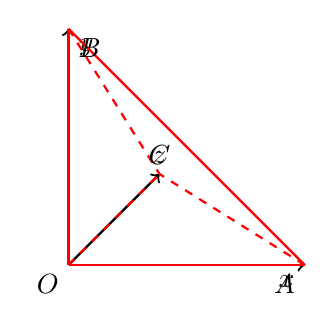
\begin{tikzpicture}
  % Axes
  \draw[->, thick] (0,0,0) -- (3,0,0) node[anchor=north east] {$x$};
  \draw[->, thick] (0,0,0) -- (0,3,0) node[anchor=north west] {$y$};
  \draw[->, thick] (0,0,0) -- (0,0,-3) node[anchor=south] {$z$};
  
  % Points
  \coordinate (O) at (0,0,0);
  \coordinate (A) at (3,0,0);
  \coordinate (B) at (0,3,0);
  \coordinate (C) at (0,0,-3);
  
  % Triangle edges
  \draw[thick, red] (O) -- (A);
  \draw[thick, red] (O) -- (B);
  \draw[thick, red,dashed] (O) -- (C);
  \draw[thick, red] (A) -- (B);
  \draw[thick, red,dashed] (B) -- (C);
  \draw[thick, red, dashed] (A) -- (C);
  
  % Labels
  \node[anchor=north east] at (A) {$A$};
  \node[anchor=north west] at (B) {$B$};
  \node[anchor=south] at (C) {$C$};
  \node[anchor=north east] at (O) {$O$};
\end{tikzpicture}
\end{document}
